\mode<presentation>
{
  \usetheme{Boadilla}
}

%\usepackage[english]{babel}
\usepackage[utf8]{inputenc}

% Note: using version 2.0-alpha3
\usepackage[cache]{minted}
\setminted{frame=single}

% Hour-long talk

\title[Exploring type-directed TDD w/FizzBuzz]{Exploring type-directed, test-driven development}
\subtitle{A case study using FizzBuzz}
\author{Franklin Chen \\ \url{http://franklinchen.com/}}
\date[\href{http://www.pghtechfest.com/}{Pittsburgh TechFest 2014}]{June 7, 2014 \\ \href{http://www.pghtechfest.com/}{Pittsburgh TechFest 2014}}

\subject{Talks}

\AtBeginSection[]
{
  \begin{frame}<beamer>{Outline}
    \tableofcontents[currentsection,subsectionstyle=hide]
  \end{frame}
}

\begin{document}

\maketitle

\begin{abstract}
  An expressive static type system is one of the most joyful and
  powerful tools for prototyping, designing, and maintaining
  programs. In this performance-theatrical presentation, I will
  provide a taste of how to use types, in conjunction with tests, to
  drive iterative development of a particular program, the famous
  FizzBuzz problem. We will solve generalizations of this problem,
  changing and adding requirements, to illustrate the pleasures and
  benefits of ``type thinking''.

  The Scala language will be used as the vehicle for this
  demonstration, but the techniques apply immediately to any
  industrial-strength statically typed language, such as Haskell,
  OCaml, F\#, Rust, and most recently, Swift.

  (Note: this presentation will use live human volunteers to play the
  roles of various programming concepts.)
\end{abstract}

\begin{frame}
  \titlepage
\end{frame}

\section*{Outline}

\begin{frame}{Outline}
  \tableofcontents[subsectionstyle=hide]
\end{frame}

% Since this a solution template for a generic talk, very little can
% be said about how it should be structured. However, the talk length
% of between 15min and 45min and the theme suggest that you stick to
% the following rules:  

% - Exactly two or three sections (other than the summary).
% - At *most* three subsections per section.
% - Talk about 30s to 2min per frame. So there should be between about
%   15 and 30 frames, all told.

\section{Introduction}

\subsection{Goals}

\begin{frame}{Goals of this presentation}
  \begin{itemize}
  \item Give a taste of a \alert{practical} software development \alert{process} that is:
    \begin{itemize}
    \item \alert{test}-driven
    \item \alert{type}-directed
    \end{itemize}
  \item Show everything for real (using Scala):
    \begin{itemize}
    \item project build process
    \item testing frameworks
    \item all the code
    \end{itemize}
  \item Use \texttt{FizzBuzz} because:
    \begin{itemize}
    \item problem: easy to understand
    \item modifications: easy to understand
    \item fun!
    \end{itemize}
  \item Encourage you to explore a modern typed language
    \begin{itemize}
    \item This Monday, Apple ditched Objective C for its new language \href{https://developer.apple.com/swift/}{Swift}!
      
\includegraphics[height=0.75cm]{swift-hero.png}
    \item Complete Swift code will shown at the end; \href{https://github.com/densh/talks/blob/master/swift-vs-scala-211-2014-06-03/Swift\%20vs\%20Scala\%202.11.pdf}{looks a lot like Scala}.
    \end{itemize}
  \end{itemize}
\end{frame}

\subsection{Test-driven development (TDD)}

\begin{frame}{Test-driven development (TDD)}
  \begin{itemize}
  \item Think.
  \item Write a test that \textcolor{red}{fails}.
  \item Write code until test \textcolor{green}{succeeds}.
  \item Repeat, and \textcolor{green}{refactor} as needed.
  \end{itemize}

  \begin{block}{\href{http://martinfowler.com/articles/is-tdd-dead/}{Is TDD dead?}}
    Short answer: No.
  \end{block}
\end{frame}

\subsection{Type systems}

\begin{frame}{Type systems}
  \begin{block}{What is a type system?}
    A \alert{syntactic} method to \alert{prove} that bad things can't happen.
  \end{block}

  \begin{block}{``Debating'' types ``versus'' tests?}
    \begin{itemize}
    \item Let's use both types and tests!
    \item But: use a \alert{good} type system, not a bad one.
    \end{itemize}
  \end{block}

  \begin{block}{Some decent practical typed languages}
    \begin{itemize}
    \item \href{http://ocaml.org/}{OCaml}: 20 years old
    \item \href{http://www.haskell.org/}{Haskell}: 20 years old
    \item \href{http://www.scala-lang.org/}{Scala}: 10 years old
    \item \href{http://developer.apple.com/swift/}{Swift}: 5 days old
    \item \href{http://www.rust-lang.org/}{Rust} (still in progress)
    \end{itemize}
  \end{block}
\end{frame}

\begin{frame}<article|handout>{Poor versus decent type systems}
  \begin{block}{Poor type systems}
    \begin{itemize}
      \mode<article|handout>{
        \item (Developed using 1960s-1970s knowledge)
      }
    \item C, C++, Objective C
    \item Java
    \end{itemize}
  \end{block}

  \begin{block}{Decent type systems}
    \begin{itemize}
      \mode<article|handout>{
        \item (Developed using 1980s-1990s knowledge)
      }
    \item ML (\href{http://www.smlnj.org/}{Standard ML}, \href{http://ocaml.org/}{OCaml}, \href{http://fsharp.org/}{F\#}): I first used for work in 1995
    \item \href{http://www.haskell.org/}{Haskell}: I first used for work in 1995
    \item \href{http://www.scala-lang.org/}{Scala}: first released in 2004
    \item \href{http://developer.apple.com/swift/}{Swift}: announced by Apple on June 2, 2014!
    \item \href{http://www.rust-lang.org/}{Rust}: not yet version 1.0
    \end{itemize}
  \end{block}
\end{frame}

\section{Original FizzBuzz problem}

\subsection{Original FizzBuzz problem}

\begin{frame}{Original FizzBuzz problem}
  \begin{block}{FizzBuzz defined}
    Write a program that prints the numbers from 1 to 100.

    But for multiples of three, print ``Fizz'' instead of the number.

    And for the multiples of five, print ``Buzz''.

    For numbers which are multiples of both three and five, print ``FizzBuzz''.
  \end{block}
\end{frame}

\subsection{Starter code: main driver}

\begin{frame}[fragile]{Starter code: main driver}
  \begin{block}{
\includegraphics[height=0.75cm]{scala-logo-red-dark.png}}
    Scala: a modern \alert{object-oriented} and \alert{functional} language.
  \end{block}

  \inputminted{scala}{Main1.scala}

  \begin{itemize}
  \item Type-directed design: separate out effects (such as printing to terminal) from the real work.
  \item Type-directed feedback: compilation fails when something is not implemented yet.
  \end{itemize}
\end{frame}

\subsection{The joys of continuous compilation and testing}

\begin{frame}[fragile]{The joys of continuous compilation and testing}
  \begin{block}{
\includegraphics[height=0.75cm]{sbt-logo-orange-600x360.png}}
    \href{http://www.scala-sbt.org/}{SBT}: build tool supporting Scala, Java\dots
  \end{block}

  \begin{block}{Winning features}
    \begin{itemize}
    \item \href{http://www.scala-sbt.org/release/docs/Detailed-Topics/Triggered-Execution.html}{Source file changes trigger smart recompilation!}
    \item Source file changes trigger rerun of the tests that depend on changed code!
    \end{itemize}
  \end{block}

  \inputminted{console}{testQuick.console}
\end{frame}

\begin{frame}[fragile]{Write type-directed stub}
  \inputminted{scala}{Main2.scala}

  \begin{block}{Write wanted type signature}
    \mintinline{scala}{???} is convenient for stubbing.
    \begin{itemize}
    \item In Scala standard library
    \item Just performs: \mintinline{scala}{throw new NotImplementedError}
    \end{itemize}
  \end{block}
\end{frame}

\subsection{Write acceptance test (simplified)}

\begin{frame}[fragile]{Write acceptance test (simplified)}
  \begin{block}{
\includegraphics[height=0.75cm]{specs2.png}}
    \href{http://specs2.org/}{Specs2}: a fine testing framework for Scala, Java\dots
  \end{block}

  \inputminted{scala}{MainSpec1.scala}

  \mode<article>{
    A realistic acceptance test would involve handling I/O, but an elegant
    technique for modularizing that,
    \href{https://github.com/scalaz/scalaz-stream}{\texttt{scalaz-stream}},
    is outside the scope of this presentation.
  }
\end{frame}

\begin{frame}<article|handout>[fragile]{TDD in Swift}
  \inputminted{ocaml}{MainSpec1.swift}
\end{frame}

\begin{frame}[fragile]{Test passes type check, but fails}
  Incremental compilation/testing kicks in:

  \inputminted{console}{testQuick2.console}
\end{frame}

\begin{frame}[fragile]{Outside-in: for a \mintinline{scala}{FizzBuzz} unit}
  Types are shapes to assemble logically.

  \inputminted[gobble=2]{scala}{Main4.scala}

  \begin{itemize}
  \item \mintinline{scala}{start.to(end): Seq[Int]}, where \href{http://www.scala-lang.org/api/2.11.0/index.html\#scala.collection.Seq}{\mintinline{scala}{Seq[_]}} is a \alert{type constructor} that, given a type \mintinline{scala}{A}, returns a type of \mintinline{scala}{Seq[A]}.
  \item For any value of type \mintinline{scala}{Seq[A]}, \mintinline{scala}{map: (A => B) => Seq[B]}.
  \begin{center}
    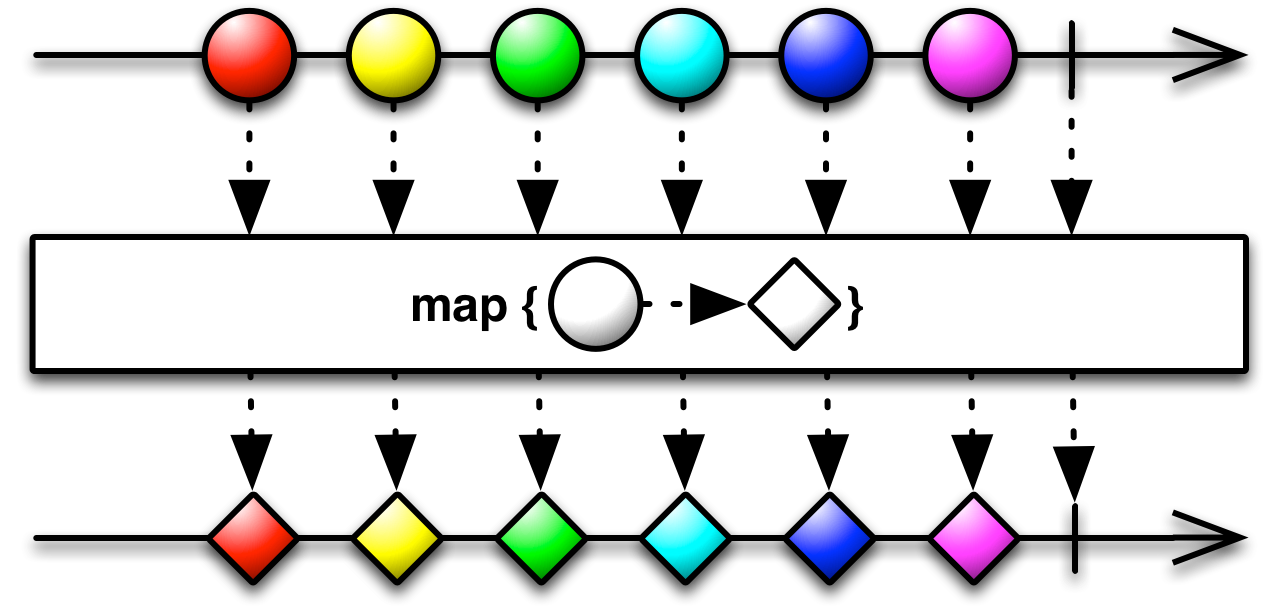
\includegraphics[height=2.5cm]{map.png}
  \end{center}
  \item Therefore: need to implement function \mintinline{scala}{FizzBuzz.evaluate: Int => String}.
  \end{itemize}
\end{frame}

\begin{frame}<article|handout>[fragile]{Swift version of driver}
  \inputminted{ocaml}{Main4.swift}
\end{frame}

\subsection{Test-driven units}

\begin{frame}[fragile]{Implement new \mintinline{scala}{FizzBuzz} module}
  A failing acceptance test drives \alert{discovery} of
  \begin{itemize}
  \item A \alert{unit}, \mintinline{scala}{FizzBuzz}
  \item A function with a particular type,
    \mintinline{scala}{Int => String}
  \end{itemize}

  \inputminted{scala}{FizzBuzz1.scala}

  \begin{block}{\alert{Types} are better than \alert{comments} as \alert{documentation}!}
    Comments are not checkable, unlike types and tests.
  \end{block}
\end{frame}

\begin{frame}[fragile]{First part of \alert{unit test}: example-based}
  Manually write some \alert{examples}.

  \inputminted{scala}{FizzBuzzSpec1.scala}
\end{frame}

\subsection{Property-based tests}

\begin{frame}[fragile]{The joy of property-based tests}
    \begin{block}{
\includegraphics[height=0.75cm]{logo_forall_h61.png}
\includegraphics[height=0.75cm]{logo_scalacheck_h61.png}}
      \href{http://scalacheck.org/}{ScalaCheck}: a framework for writing \alert{property-based} tests.
  \end{block}

  \inputminted{scala}{FizzBuzzSpec2.scala}

  \begin{block}{Winning features}
    \begin{itemize}
    \item Auto-generates \alert{random} tests for each property (100 by default).
    \item \alert{Type-driven}: here, generates random \mintinline{scala}{Int} values.
    \end{itemize}
  \end{block}
\end{frame}

\begin{frame}<article|handout>{Property-based testing for Swift?}
  I hope someone writes a property-based testing framework for Swift!
\end{frame}

\begin{frame}[fragile]{Property-based tests (continued)}
  The other three properties of interest:

  \inputminted{scala}{FizzBuzzSpec3.scala}
\end{frame}

\subsection{Solving the FizzBuzz problem}

\begin{frame}[fragile]{A buggy and ugly solution}
  \inputminted[gobble=2]{scala}{FizzBuzzIf.scala}

  \inputminted{console}{testQuick3.console}
\end{frame}

\begin{frame}{Booleans are evil!}
\begin{block}{\href{http://en.wikiquote.org/wiki/Colossal\_Cave\_Adventure}{Maze of twisty little conditionals, all different}}
  \begin{center}
    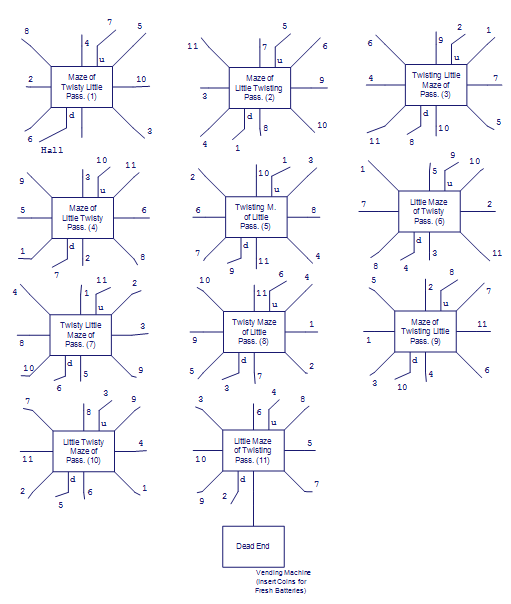
\includegraphics[height=3cm]{dmaze.png}
  \end{center}

  \begin{itemize}
  \item Too easy to write incorrect sequences of nested, combined conditionals.
  \item \href{http://existentialtype.wordpress.com/2011/03/15/boolean-blindness/}{Overuse of Booleans} is a type \alert{smell}.
  \end{itemize}
  \end{block}
\end{frame}

\begin{frame}<article|handout>{Why booleans are evil}
  \begin{block}{No help from type system}
    \begin{itemize}
    \item Conditions can be arbitrary: depend on \alert{any} combination of data.
    \item Multiple conditions: combinatorial explosion (two conditions led to four cases).
    \item Possibly overlapping conditions: order dependency subtleties.
    \item Possibly duplicated checking of the some condition.
    \end{itemize}
  \end{block}
\end{frame}

\begin{frame}[fragile]{Pattern matching organizes information}
  \inputminted[gobble=2]{scala}{FizzBuzz2.scala}

  \begin{block}{Winning features}
    \begin{itemize}
    \item Visual \alert{beauty} and clarity.
    \item No duplicated conditionals.
    \item No ordering dependency.
    \item \alert{Type checker} verifies \alert{full coverage} of cases.
    \end{itemize}
  \end{block}
\end{frame}

\begin{frame}[fragile]{Example of non-exhaustive pattern matching}
  \inputminted[gobble=2]{scala}{FizzBuzz2Bad.scala}

  \inputminted{console}{testQuick4.console}
\end{frame}

\begin{frame}<article|handout>[fragile]{Swift digression: pattern matching}
  The same solution, in Swift:

  \inputminted{ocaml}{FizzBuzz2.swift}
\end{frame}

\begin{frame}[fragile]{Acceptance test passes}

  \inputminted{console}{testQuick5.console}

  \begin{block}{Done?}
    No. Client wants more features.
  \end{block}
\end{frame}

\section{FizzBuzz 2: user configuration}

\subsection{Adding new features}

\begin{frame}{Adding new features}
  \begin{block}{Client wants to:}
    \begin{itemize}
    \item Choose two \alert{arbitrary} divisors in place of \mintinline{scala}{3} and \mintinline{scala}{5}
      \begin{itemize}
      \item such as \mintinline{scala}{4} and \mintinline{scala}{7}
      \end{itemize}
    \item Choose other \alert{arbitrary} words in place of \mintinline{scala}{"Fizz"} and \mintinline{scala}{"Buzz"}
      \begin{itemize}
      \item such as \mintinline{scala}{"Moo"} and \mintinline{scala}{"Quack"}

      \end{itemize}
    \end{itemize}
  \end{block}
\end{frame}

\subsection{Type-driven refactoring}

\begin{frame}{Type-driven refactoring}
  \begin{block}{Types mean: refactoring is much more fun!}
  \begin{itemize}
  \item Add \alert{new} tests.
  \item Change types and code: to make new tests \alert{type check}.
  \item \alert{Refactor} original code and tests: use new APIs.
  \item Keep passing the \alert{old} tests.
  \item Delay writing code for new features.
  \end{itemize}
  \end{block}
\end{frame}

\begin{frame}[fragile]{More features means more types}
  Change \mintinline{scala}{FizzBuzz.evaluate} to \mintinline{scala}{Defaults.fizzBuzzer}:
  \inputminted[gobble=2]{scala}{Main5.scala}

  Add new types to \mintinline{scala}{FizzBuzz} module:
  \inputminted[gobble=2]{scala}{FizzBuzz3.scala}
\end{frame}

\begin{frame}[fragile]{Extract original default configuration}
  \inputminted{scala}{Defaults1.scala}
\end{frame}

\begin{frame}[fragile]{More types means more tests}
  Write new property-based test over \alert{arbitrary} user configurations:
  \inputminted[gobble=2]{scala}{FizzBuzzSpec6.scala}
\end{frame}

\subsection{Refining types}

\begin{frame}[fragile]{Problem: coarse \mintinline{scala}{Config} type}
  \inputminted{console}{testQuick6.console}

  \begin{itemize}
  \item \mintinline{scala}{0} as a divisor \alert{crashes}!
  \item We discovered client's \alert{underspecification}.
  \item Client says: meant to allow only divisors within \mintinline{scala}{2} and \mintinline{scala}{100}.
  \end{itemize}

  We need to:
  \begin{itemize}
  \item Add runtime \alert{validation} when \alert{constructing} \mintinline{scala}{Config}.
  \item Refine \mintinline{scala}{Config} random generator.
  \end{itemize}
\end{frame}

\subsection{Validation}

\begin{frame}[fragile]{Add (runtime) validation}
  \alert{Runtime} precondition contract: Scala's \mintinline{scala}{require} (throws exception on failure):

  \inputminted[gobble=2]{scala}{FizzBuzz3Validate.scala}
\end{frame}

\begin{frame}{A note on exceptions and types}
  \begin{itemize}
  \item \href{http://blog.jessitron.com/2013/06/whats-dirtier-than-comments-exceptions.html}{Exceptions are evil} because they escape the type system.
  \item In real life, I prefer to use a principled \alert{type-based} validation system, such as \href{http://eed3si9n.com/learning-scalaz/Validation.html}{Scalaz}.
  \item Note: Swift does not have exceptions, so expect some type-based libraries to emerge!
  \end{itemize}
\end{frame}

\begin{frame}<article|handout>[fragile]{Data validation can be critical!}
  \begin{block}{Digression: two ways to prevent \href{http://heartbleed.com/}{Heartbleed}}
    \begin{itemize}
    \item Instead of C: use a \href{http://en.wikipedia.org/wiki/Dependent_type}{dependently typed} safe systems language such as \href{http://www.ats-lang.org/}{ATS} for \href{http://bluishcoder.co.nz/2014/04/11/preventing-heartbleed-bugs-with-safe-languages.html}{compile-time TDD}.
    \item Even with C: use \href{http://martinfowler.com/articles/testing-culture.html}{good validation and testing practices}.
      \begin{itemize}
      \item A weaker type system is not an \alert{excuse} to skip
        write tedious validation code or tests!
      \end{itemize}
    \end{itemize}
  \end{block}
\end{frame}

\begin{frame}[fragile]{Improve \mintinline{scala}{Config} random generator}
  \inputminted[gobble=2]{scala}{FizzBuzzSpec7.scala}
\end{frame}

\begin{frame}[fragile]{New test runs further, stills fails}
  Refactor old code to \mintinline{scala}{FizzBuzz.compile}, to pass old tests and new test.

  \inputminted{scala}{FizzBuzz3Compile.scala}
\end{frame}

\section{FizzBuzz 3: \texttt{FizzBuzzPop} and beyond}

\subsection{Generalize to more than two divisors}

\begin{frame}[fragile]{Generalizing to more than two divisors}
  \begin{block}{Client wants \texttt{FizzBuzzPop}!}
  \begin{itemize}
  \item Given three divisors (such as 3, 5, 7).
  \item Given three words (such as \mintinline{scala}{"Fizz"}, \mintinline{scala}{"Buzz"}, \mintinline{scala}{"Pop"}).
    \mode<article|handout>{
  \item Compile to evaluator that given an integer prints:
    \begin{itemize}
    \item either a string combining a subset of the three words, or
    \item a numerical string if the integer is not a multiple of any of the three divisors
    \end{itemize}
    }
  \item Example: \mintinline{scala}{21} should output \mintinline{scala}{"FizzPop"}.
  \end{itemize}
  \end{block}
\end{frame}

\begin{frame}<article|handout>{Thought-driven development}
    Software development is not primarily about \alert{coding}, but \alert{thinking}.

  \begin{itemize}
  \item Deep fact: solving a more general problem is often easier than solving the specific problem.
  \item There are four important numbers in the Universe:
    \begin{description}
    \item[0] emptiness
    \item[1] existence
    \item[2] other (relationship)
    \item[many] community
    \end{description}
  \end{itemize}
\end{frame}

\subsection{More features means more tests and types (again)}

\begin{frame}[fragile]{More features means more tests}
  Write new tests for new \mintinline{scala}{Defaults.fizzBuzzPopper}:

  \inputminted[gobble=2]{scala}{FizzBuzzSpec5.scala}

  Change configuration: to \mintinline{scala}{Seq} of pairs, instead of just two:
  \inputminted[gobble=2]{scala}{Defaults2.scala}
\end{frame}

\begin{frame}[fragile]{More tests means more (or changed) types}
  \inputminted{console}{testQuick8.console}

  Change \alert{type} \mintinline{scala}{Config} to allow a sequence of pairs:

  \inputminted[gobble=2]{scala}{FizzBuzz3Seq.scala}

  \mode<article|handout>{
    Note how our iterative development process promotes \alert{reuse} (here, of validation logic).
  }
\end{frame}

\begin{frame}[fragile]{Fix remaining type errors}
  Refactoring reveals need to implement case of more than two divisors.

  \inputminted[gobble=2]{scala}{FizzBuzz3SeqCompile.scala}
\end{frame}

\begin{frame}<article|handout>{General observations}
  \begin{itemize}
  \item Return a sum of a subset of the configured words, if there is any divisor match.
  \item If there is \alert{no} divisor match, return the numerical string.
  \end{itemize}
\end{frame}

\begin{frame}[fragile]{More computation means more types}
  Compile each divisor to a ``rule'' that awaits input.

  \inputminted[gobble=2]{scala}{FizzBuzz4.scala}

  \begin{block}{\texttt{FizzBuzz} demo time!}
    \begin{itemize}
    \item Two volunteers: to play role of \mintinline{scala}{Rule}.
    \item One volunteer: to combine sub-results.
    \end{itemize}
  \end{block}
\end{frame}

\subsection{Demo}

\begin{frame}<article|handout>{Demo explanation}
  \begin{itemize}
  \item Given a sequence of rules and an integer: apply all the rules to the integer, then combine the partial results.
  \end{itemize}

\end{frame}

\begin{frame}[label=first-general,fragile]{Assemble the types}
  \inputminted[gobble=2]{scala}{FizzBuzz5.scala}
\end{frame}

\begin{frame}[fragile]{A note on \mintinline{scala}{reduce}}
  For any value of type \mintinline{scala}{Seq[A]}, \mintinline{scala}{reduce: ((A, A) => B) => B}.
  \begin{center}
    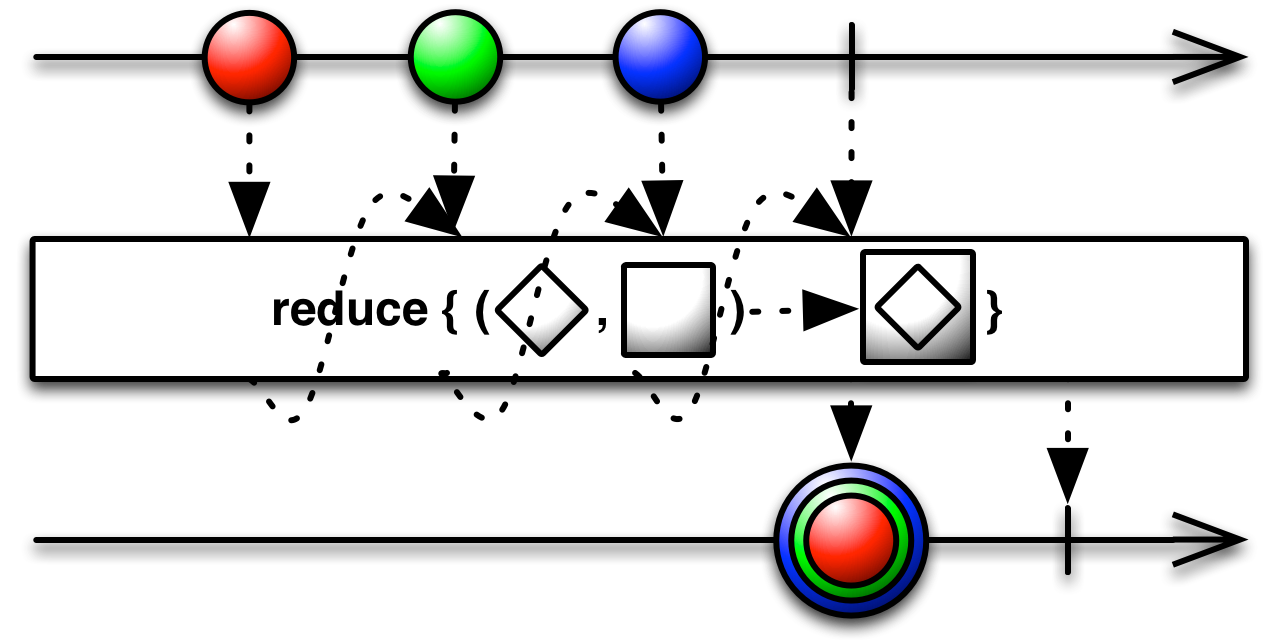
\includegraphics[height=2.5cm]{reduce.png}
  \end{center}

  Example: for \mintinline{scala}{Seq[String]}, reduction with string concatenation \mintinline{scala}{+} returns the concatenation of all the strings in the sequence.
\end{frame}

\begin{frame}[fragile]{Test failure: coarse types again}
  \inputminted[gobble=2]{console}{testQuick9.console}

  \begin{block}{Demo time!}
    \begin{itemize}
    \item Configuration: \mintinline{scala}{Seq(3 -> "", 5 -> "Buzz")}
    \item Input: \mintinline{scala}{2}
    \item Output: should be \mintinline{scala}{""}
    \item Output was: \mintinline{scala}{"2"}
    \end{itemize}
  \end{block}
\end{frame}

\againframe<beamer>{first-general}

\begin{frame}[fragile]{Property-based testing rescued us again!}
  \begin{block}{Be honest: would you have caught this bug manually?}
    \begin{itemize}
    \item I didn't.
    \item I never wrote \texttt{FizzBuzzPop} examples testing empty strings.
    \item Property-based testing reveals \alert{unexpected} corner cases.
      \begin{itemize}
      \item (Empty ``fizz'' and ``buzz'' word strings).
      \end{itemize}
    \end{itemize}
  \end{block}
\end{frame}

\subsection{\mintinline{scala}{Option[A]} type}

\begin{frame}{An empty string is \alert{not} equivalent to no string}
  \begin{block}{Presence of something ``empty'' is \alert{not} equivalent to no thing.}
    Sending someone an empty email versus not sending any email.
  \end{block}
  
  Many programming languages get this wrong.
\end{frame}

\begin{frame}[fragile]{\mintinline{scala}{Option[A]} type}

  \mintinline{scala}{Option[A]} is one of two possibilities:
  \begin{itemize}
  \item \mintinline{scala}{None}
  \item \mintinline{scala}{Some(a)} wraps a value \mintinline{scala}{a} of type \mintinline{scala}{A}.
  \end{itemize}

  For example, \mintinline{scala}{Some("")} is not the same as \mintinline{scala}{None}.

  \inputminted{scala}{OptionExample1.scala}
\end{frame}

\begin{frame}[fragile]{Cleaning up the types}
  \inputminted[gobble=2]{scala}{FizzBuzz6.scala}

  Useful type errors:

  \inputminted[gobble=2]{console}{testQuick10.console}
\end{frame}

\begin{frame}[fragile]{Fix the type errors: our rule builder}
  \inputminted[gobble=2]{scala}{FizzBuzz7Rule.scala}

  \begin{block}{Demo time!}
    \begin{itemize}
    \item (Instructions: circle what you write to wrap it with \mintinline{scala}{Some})
    \item Configuration: \mintinline{scala}{Seq(3 -> "", 5 -> "Buzz")}
    \item Input: \mintinline{scala}{2}
    \item Output: should be \mintinline{scala}{""}
    \end{itemize}
  \end{block}
\end{frame}

\begin{frame}[fragile]{Fix the type errors: our compiler}
  \inputminted[gobble=2]{scala}{FizzBuzz7.scala}

  \begin{itemize}
  \item We need to write: \mintinline{scala}{addOption}
  \item Scala standard library provides: \mintinline{scala}{getOrElse}
  \end{itemize}
\end{frame}

\begin{frame}[fragile]{``Addition'' for \mintinline{scala}{Option[String]}}
  \inputminted[gobble=2]{scala}{FizzBuzz8.scala}
\end{frame}

\begin{frame}[fragile]{Getting \mintinline{scala}{A} back out of \mintinline{scala}{Option[A]}}
  \begin{block}{Do not lose information!}
    \mintinline{scala}{getOrElse} inspects the \mintinline{Option[A]} value and either
    \begin{itemize}
    \item returns the value \mintinline{scala}{v} inside a \mintinline{scala}{Some(v)},
    \item or else returns the specific default value.
    \end{itemize}
  \end{block}
\end{frame}

\begin{frame}<article|handout>[fragile]{Swift has two option types}
  Swift calls them ``optionals''.

  \begin{block}{Normal optional type}
    \begin{itemize}
    \item \mintinline{ocaml}{A?} is a type for each type \mintinline{scala}{A}.
    \item Must unwrap explicitly.
    \end{itemize}
  \end{block}

  \begin{block}{Implicit unwrapped optional type}
    \begin{itemize}
    \item \mintinline{ocaml}{A!} is a type for each type \mintinline{scala}{A}.
    \item Unfortunate type hole:
      \begin{quote}
        If you try to access an implicitly unwrapped optional when it
        does not contain a value, you will trigger a runtime error.
      \end{quote}
    \end{itemize}
  \end{block}
\end{frame}

\begin{frame}[fragile]{The same thing, in Swift}
  \inputminted{ocaml}{FizzBuzz8.swift}
\end{frame}

\subsection{Transform information; don't destroy it}

\begin{frame}[fragile]{Transform information; don't destroy it}
  Did you notice? Our new code no longer uses \mintinline{scala}{if}.

  \begin{block}{Bug cause: destroying information, using \mintinline{scala}{if}} 
    \begin{itemize}
    \item Building a rule: \mintinline{scala}{if (i % n == 0) word else ""}
    \item Obtaining a final string answer: \mintinline{scala}{if (combined == "") i.toString else combined}
    \end{itemize}
  \end{block}

  \begin{block}{Transforming information}
    \begin{itemize}
    \item To \mintinline{scala}{Option[String]}: \mintinline{scala}{(i % n == 0).option(word)}
    \item To \mintinline{scala}{String}: \mintinline{scala}{combinedOption.getOrElse(i.toString)}
    \end{itemize}
  \end{block}

  \begin{block}{Type-directed design tip}
    We could have saved trouble \alert{up front}, by using precise \alert{types}.
    \begin{itemize}
    \item Avoid \mintinline{scala}{if}, when possible.
    \item Avoid \mintinline{scala}{String} (but required at I/O boundaries of program).
    \end{itemize}
  \end{block}
\end{frame}

\begin{frame}[fragile]{Bonus: the final code in Swift}
  \inputminted{ocaml}{FizzBuzzFinal.swift}
\end{frame}


\section{Parallel \texttt{FizzBuzz}}

\begin{frame}[fragile]{Parallelism}
  \begin{itemize}
  \item Use of \alert{map}: parallelizable; there are high-performance \href{http://scala-blitz.github.io/}{parallel collections} for Scala.
  \item Use of \alert{reduce}: parallelizable because of the monoid property:
  \begin{block}{\mintinline{scala}{Option[String]} is a \href{http://en.wikipedia.org/wiki/Monoid}{Monoid}}
  \begin{itemize}
  \item There is an identity element (\mintinline{scala}{None}).
  \item There is a binary associative operator (\mintinline{scala}{addOption}).
  \item \href{http://www.michael-noll.com/blog/2013/12/02/twitter-algebird-monoid-monad-for-large-scala-data-analytics/}{Fantastically important in practice!}
  \end{itemize}
  \end{block}

  \begin{block}{Demo time!}
    \begin{itemize}
    \item Configuration: \mintinline{scala}{Seq(3 -> "Fizz", 5 -> "Buzz", 7 -> "Pop", 2 -> "Boom")}
    \item Input: \mintinline{scala}{42}
    \item Output: \mintinline{scala}{"FizzPopBoom"}
    \end{itemize}
  \end{block}
  \end{itemize}

\end{frame}

\begin{frame}[fragile]{Final parallelized code}
  \inputminted[gobble=2]{scala}{FizzBuzz9.scala}

  \begin{block}{Coding style tip}
    This level of conciseness is not always best: maybe too ``clever''?
  \end{block}
\end{frame}

\begin{frame}<article|handout>{Parallelism for Swift?}
  I expect people to develop libraries for parallelism in Swift.
\end{frame}

\begin{frame}{Parallelism summary}
  We discovered a theoretical speedup for generalized \texttt{FizzBuzz}:
  \begin{itemize}
  \item Sequential: $O(n)$
  \item Parallel: $O(\log n)$ (given $\log n$ processors, and omitting some technical subtleties)
  \end{itemize}

  Also, driver outer loop can be sped up:
  \begin{itemize}
  \item Sequential loop on 1 to $m$: $O(m)$
  \item Parallel loop: $O(1)$ (given $m$ processors)
  \end{itemize}
\end{frame}

\begin{frame}{Future work}
  \begin{itemize}
  \item Asynchronous
  \item Real-time
  \item Interactive
  \end{itemize}
\end{frame}

\section{Conclusion}

\begin{frame}{Conclusion}
  \begin{itemize}
  \item \alert{Tests} are great.
  \item \alert{Types} are great.
  \item Tests and types work hand in hand, driving design and program evolution.
  \item Modern typed languages such as Scala promote fun, correct programming!
  \item It's a great time to be learning and using a modern typed language: Apple ditched Objective C for Swift.
  \end{itemize}

  \begin{block}{Code, slides, article}
    \begin{itemize}
    \item Go to  \url{https://github.com/franklinchen/talk-on-type-directed-tdd-using-fizzbuzz}
    \item The \href{https://github.com/FranklinChen/talk-on-type-directed-tdd-using-fizzbuzz/blob/master/doc/article.pdf}{article} has more detail omitted in the presentation.
    \item The hyperlinks in all provided PDFs are clickable.
    \item The Swift code: \url{https://github.com/franklinchen/fizzbuzz-swift}
    \end{itemize}
  \end{block}
\end{frame}

\appendix

\section*{\appendixname}

\begin{frame}{Some free online courses on modern typed functional programming}
  \begin{itemize}
  \item Using Scala: \href{http://www.coursera.org/course/progfun}{Functional Programming Principles in Scala} on Coursera, taught by Martin Odersky (inventor of Scala)
  \item Using Haskell: \href{http://www.edx.org/course/delftx/delftx-fp101x-introduction-functional-2126}{Introduction to Functional Programming} on EdX, taught by Erik Meijer (Haskell hero)
  \end{itemize}
\end{frame}

\end{document}

%%% Local Variables: 
%%% mode: latex
%%% TeX-master: "presentation"
%%% End: 
